\documentclass[]{report}
\usepackage{graphicx, float}
\usepackage[export]{adjustbox}

\title{\centering CSP334 : Computer Networks \\Lab Assignment No 1\\Assignment on Wireshark}
\author{\LARGE Sahil\\2016UCS0008}

% to use proper section numbering in the report type 
\renewcommand{\thesection}{\arabic{section}}

\begin{document}

\maketitle

%%%%%%%%%%%%%%%%%%%%%%%%%%%%%%%%%%%%%%%%%%%%%%%%
\section{Network Interface:}


%%%%%%%%%%%%%%%%%%%%%%%%%%%%%%%%%%%%%%%%%%%%%%%%
\section{Application Layer protocol used:}


%%%%%%%%%%%%%%%%%%%%%%%%%%%%%%%%%%%%%%%%%%%%%%%%
\section{Other protocols used:}


%%%%%%%%%%%%%%%%%%%%%%%%%%%%%%%%%%%%%%%%%%%%%%%%
\section{IPA of source and destination:}


%%%%%%%%%%%%%%%%%%%%%%%%%%%%%%%%%%%%%%%%%%%%%%%%
\section{Class of IPA:}


%%%%%%%%%%%%%%%%%%%%%%%%%%%%%%%%%%%%%%%%%%%%%%%%
\section{Frame: Information about packet}


%%%%%%%%%%%%%%%%%%%%%%%%%%%%%%%%%%%%%%%%%%%%%%%%
\section{Interface ID and address of interface:}


%%%%%%%%%%%%%%%%%%%%%%%%%%%%%%%%%%%%%%%%%%%%%%%%
\section{Time taken between HTTP GET and HTTP OK reply:}


%%%%%%%%%%%%%%%%%%%%%%%%%%%%%%%%%%%%%%%%%%%%%%%%
\section{HTTP GET and OK messages:}


%%%%%%%%%%%%%%%%%%%%%%%%%%%%%%%%%%%%%%%%%%%%%%%%
\section{Destination physical address of the first packet captured and device it belongs to:}


%%%%%%%%%%%%%%%%%%%%%%%%%%%%%%%%%%%%%%%%%%%%%%%%
\section{Bytes of header in the first frame:}


%%%%%%%%%%%%%%%%%%%%%%%%%%%%%%%%%%%%%%%%%%%%%%%%
\section{How to know if Ethernet header contains an IP packet?}


%%%%%%%%%%%%%%%%%%%%%%%%%%%%%%%%%%%%%%%%%%%%%%%%
\section{How to know if the first packet captured has TCP or UDP as transport protocol by looking at the IP header?}


%%%%%%%%%%%%%%%%%%%%%%%%%%%%%%%%%%%%%%%%%%%%%%%%
\section{Source and destination ports in the SYN, ACK:}


%%%%%%%%%%%%%%%%%%%%%%%%%%%%%%%%%%%%%%%%%%%%%%%%
\section{Server Hello message has 1 as relative sequence number and 185 as relative acknowledgement number:}


%%%%%%%%%%%%%%%%%%%%%%%%%%%%%%%%%%%%%%%%%%%%%%%%
\section{First sequence number sent by the server to the client:}


%\begin{figure}[H]
%	\vspace{0pt}
%	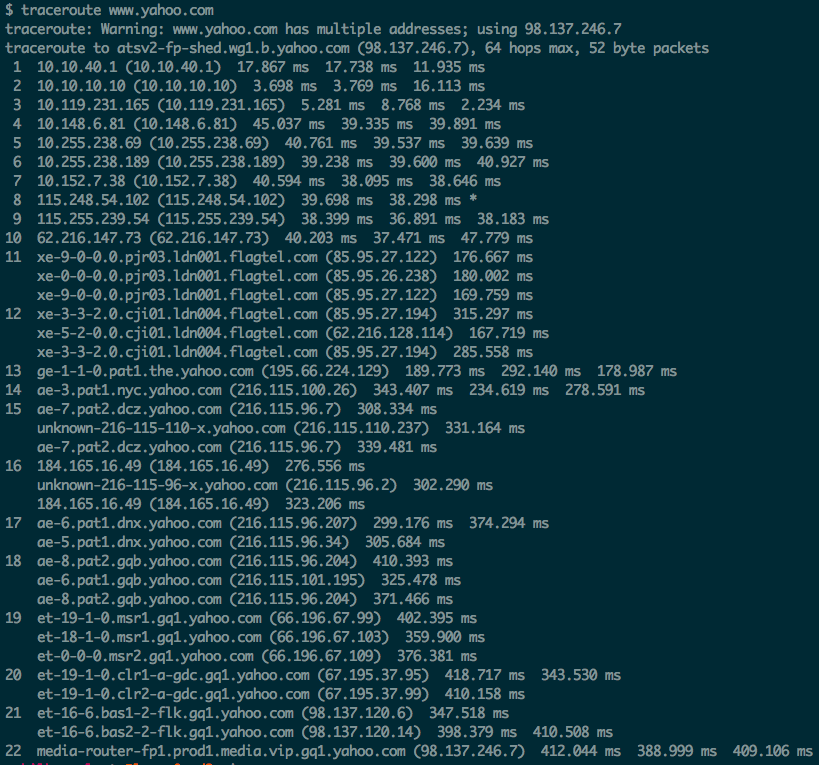
\includegraphics[height = 350pt, keepaspectratio]{Snapshots/exe2/exe2_2.png}
%\end{figure}

\end{document}